\documentclass[a4paper,12pt]{article} % тип документа

%  Русский язык
\usepackage[T2A]{fontenc}			% кодировка
\usepackage[utf8]{inputenc}			% кодировка исходного текста
\usepackage[english,russian]{babel}	% локализация и переносы

\usepackage{graphicx, scalerel}               % импорт изображений
\usepackage{wrapfig}                % обтекаемые изображения
\graphicspath{{pictures/}}          % обращение к подкаталогу с изображениями
\usepackage[14pt]{extsizes}         % для того чтобы задать нестандартный 14-ый размер шрифта
\usepackage[warn]{mathtext}         % русский язык в формулах
\usepackage{indentfirst}            % indent first
\usepackage[margin = 25mm]{geometry}% отступы полей
\usepackage[table,xcdraw]{xcolor}   % таблицы
\usepackage{amsmath,amsfonts,amssymb,amsthm,mathtools} % Математика
\usepackage{wasysym}                % ???
\usepackage{upgreek}                % ???  
\usepackage{caption}
\usepackage{multirow}
\captionsetup{labelsep=period}
\usepackage[font=small,labelfont=bf]{caption}
\usepackage{gensymb} % degree symbol
\usepackage{tikz}
\usetikzlibrary{positioning}




\begin{document}
	
	
	\begin{center}
		
		
		\textbf{НАЦИОНАЛЬНЫЙ ИССЛЕДОВАТЕЛЬСКИЙ УНИВЕРСИТЕТ \\ <<МОСКОВСКИЙ ФИЗИКО-ТЕХНИЧЕСКИЙ ИНСТИТУТ>>}
		\vspace{13ex}
		
		\textbf{Лабораторная работа 4.3.1\\ <<Изучение дифракции света>>}
		\vspace{40ex}
		
		\normalsize{Овсянников Михаил Александрович \\ студент группы Б01-001\\ 2 курс ФРКТ\\}
	\end{center}
	
	\vfill 
	
	\begin{center}
		г. Долгопрудный\\ 
		2022 г.
	\end{center}
	
	
	\thispagestyle{empty} % выключаем отображение номера для этой страницы
	\newpage
	
	\textbf{Цель работы:} исследовать дифракцию Френеля и Фраунгофера, изучить влияние дифракции на разрешающую способность оптических инструментов.
	
	\textbf{В работе используются:} оптическая скамья, ртутная лампа, монохроматор, щели с регулируемой шириной, рамка с вертикальной нитью, двойная щель, микроскоп на поперечных салазках с микрометрическим винтом, зрительная труба
	
	\section*{А. Дифракция Френеля}
	Схема установки для наблюдения дифракции Френеля представлена на рис. 1. Световые лучи освещают щель $S_2$ и испытывают на ней дифракцию. Дифракционная картина рассматривается с помощью микроскопа $M$, сфокусированного на некоторую плоскость наблюдения $\Pi$.
	
	\begin{figure}[h!]
		\centering
		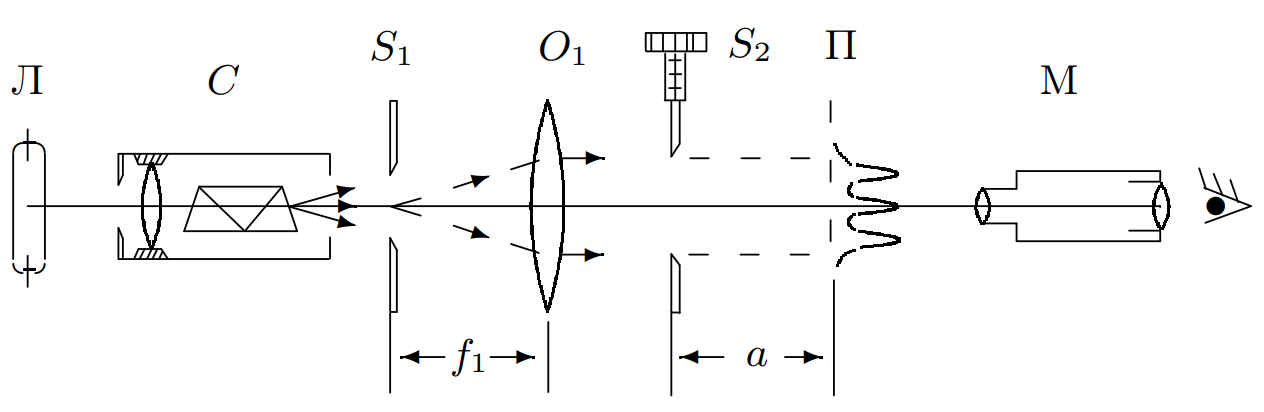
\includegraphics[scale=0.6]{Pictures/Frenel}
		\caption{Схема установки для наблюдения дифракции Френеля}
	\end{figure}

	Вид наблюдаемой дифракционной картины определяется числом Френеля $\Phi$:
	\begin{equation*}
		\Phi ^2 = \frac{D}{\sqrt{a\lambda}}.
	\end{equation*}
	
	\begin{center}
		\textbf{I. Подготовка приборов к работе}
	\end{center}

	\begin{enumerate}
		\item Соберем схему согласно рис. 1.
		
		\item Для освещения параллельным пучком щели $S_2$ установим линзу $O_1$ на расстоянии от щели $S_1$, близком к фокусному $f_1 = 10,8$ см.
		
		\item Настроим трубу на бесконечность.

		
		\item Поставим зрительную трубу за линзой $O_1$.
		Слегка перемещая линзу $O_1$ вдоль оси системы, найдем в окуляре зрительной трубы резкое изображение входной щели $S_1$. Закрепим входную щель и линзу на оптической скамье.
		
		\item Определим нуль микрометрического винта щели $S_2$: глядя сквозь щель на окно или лампу накаливания, определим момент её открытия. Далее все данные уже отсчитаны от нового нуля. Установим ширину щели 0,23 мм. Поставим щель $S_2$ за линзой $O_1$ и закрепим.
		
		\item Сфокусируем микроскоп на щель $S_2$. . Поставим микроскоп за щелью $S_2$ так, чтобы указатель продольного перемещения салазок микроскопа был расположен со стороны окуляра. Перемещая микроскоп вдоль оптической оси, найдем в окуляре резкое изображение щели $S_2$.
		
		\item Методом последовательных приближений увеличим контрастность картины.
		
		
		\begin{center}
			\textbf{II. Измерения}
		\end{center}
		
		\item Добившись наибольшей чёткости дифракционной картины, снова найдем резкое изображение щели. Запишем начальное положение микроскопа — координату по шкале продольной линейки, расположенной на оптической скамье $x_0 = 72$ см.
		
		\item Постепенно отодвигая микроскоп от щели $S_2$, заметим по шкале положение микроскопа, при котором на фоне щели видна одна темная полоса. Смещение микроскопа от первоначального положения даёт величину $a$ — расстояние от щели до плоскости наблюдения.
		
		Приближая микроскоп к щели, снимем зависимость координаты микроскопа от числа $n$ наблюдаемых тёмных полос. Результаты занесем в таблицу 1.
		
		\begin{table}[h!]
			\centering
			\begin{tabular}{|c|c|c|c|c|}
				\hline
				$n$ & $m$ & $x$, см & $a$, см & \multicolumn{1}{c|}{$2z_m$, мм} \\ \hline
				1   & 2   & 67,00   & 5,00    & 0,47                            \\ \hline
				2   & 3   & 69,00   & 3,00    & 0,44                            \\ \hline
				3   & 4   & 70,00   & 2,00    & 0,42                            \\ \hline
				4   & 5   & 70,55   & 1,45    & 0,40                            \\ \hline
				5   & 6   & 71,00   & 1,00    & 0,36                            \\ \hline
			\end{tabular}
		\caption{Зависимость $2z_m(m)$}
		\end{table}
	
		\item Измерим ширину $D$ щели $S_2$, используя микрометрический винт поперечных салазок микроскопа: $D = (0,22 \pm 0,01)$ мм.
		
		Видно, что результат совпадает с показаниями микрометрического винта щели $S_2$.
		
		
		\begin{center}
			\textbf{III. Качественные наблюдения}
		\end{center}
		
		\item Вновь сфокусируем микроскоп на щель. При небольшом удалении микроскопа от щели у её краёв появляются узкие частые полосы -- это дифракция на краю экрана.
		
		\item Закрепим микроскоп на оптической скамье и проследим за изменением дифракционной картины при уменьшении ширины щели $S_2$. Резкость картины увеличивается. В конце концов картина пропадает.
		
		\item Для исследования дифракции Френеля на препятствии поставим вместо щели $S_2$ рамку с тонкой вертикальной нитью. Настроим микроскоп на резкое изображение нити. При удалении микроскопа от нити на её фоне всегда наблюдается чётное число тёмных дифракционных полос и светлый центр.
		
		
		
		\begin{center}
			\textbf{IV. Обработка результатов}
		\end{center}
		
		\item Сравним размер зон Френеля с измеренной шириной $D$ щели $S_2$. Для этого  построим график $2z_m = f(m)$ и отложим на нем величину $D$.
		\begin{figure}[h!]
			\centering
			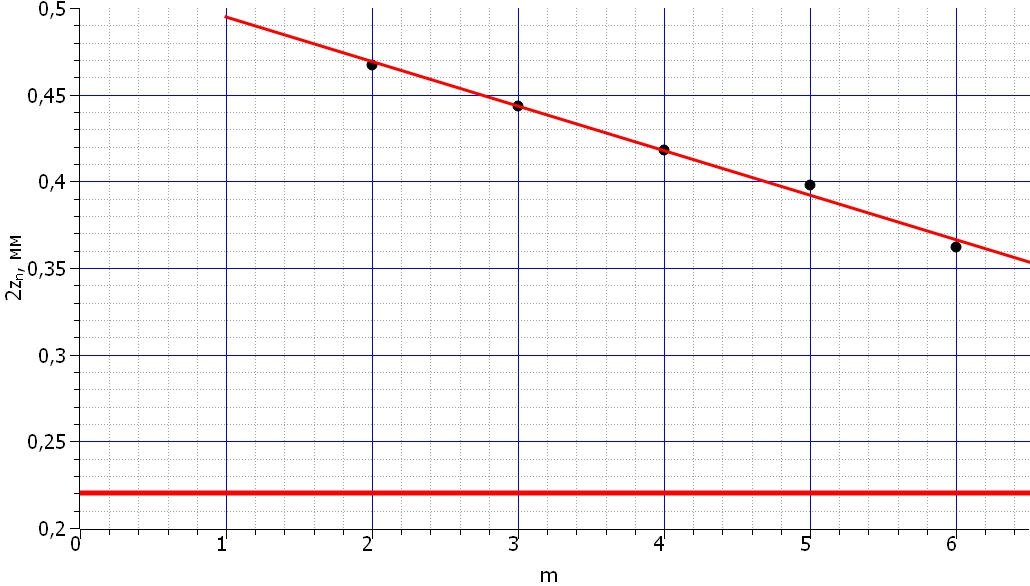
\includegraphics[scale=0.65]{Pictures/z(m)}
			\caption{Зависимость $z_m(m)$}
		\end{figure}
		
		Видно, что размер зон Френеля и ширина щели имеют одинаковые порядки, хотя последняя и меньше.
	\end{enumerate}
	
	\section*{Б. Дифракция Фраунгофера на щели}
	
	Картина дифракции резко упрощается, когда ширина щели становится значительно меньше ширины первой зоны Френеля. 
	
	Это условие всегда выполняется при достаточно большом расстоянии $a$ от щели до плоскости наблюдения. Дифракционную картину, наблюдаемую в этом случае, принято называть дифракцией Фраунгофера. Исследование такой дифракционной картины заметно облегчается, потому что упрощаются фазовые соотношения.
	
	Дифракцию Френеля и Фраунгофера можно наблюдать на одной и той же установке. Однако при обычных размерах установки дифракция Фраунгофера возникает только при очень узких щелях. Поскольку работать с такими тонкими щелями неудобно, для наблюдения дифракции Фраунгофера к схеме добавляется объектив $O_2$.
	\begin{figure}[h!]
		\centering
		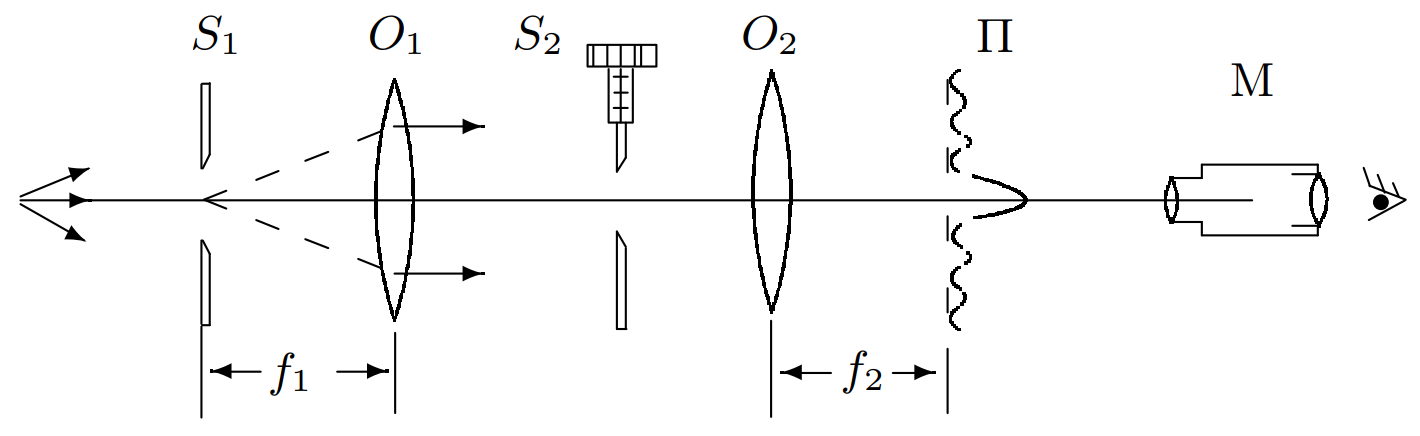
\includegraphics[scale=0.5]{Pictures/Fraungofer}
		\caption{Схема установки для наблюдения дифракции Фраунгофера на щели}
	\end{figure}
	
	
	Расстояние $X_m$ тёмной полосы от оптической оси объектива $O_2$ пропорционально фокусному расстоянию $f_2$:
	\begin{equation*}
		X_m = f_2 m \frac{\lambda}{D}.
	\end{equation*}

	\begin{center}
		\textbf{I. Настройка установки}
	\end{center}

	\begin{enumerate}
		\item Для перехода из ближней волновой зоны в дальнюю к установке, собранной по рис. 1, достаточно добавить линзу $O_2$.
		
		\item Поставьте линзу $O_2$ между щелью $S_2$ и микроскопом.
		
		Настроим микроскоп на фокальную плоскость $\Pi$ линзы. Перемещая микроскоп вдоль скамьи, найдем резкое изображение щели $S_1$.
		
		\item Поместим щель $S_2$ между линзами и подберем её ширину так, чтобы в поле зрения микроскопа появилась дифракционная картина.
Добьемся наибольшей контрастности картины.
		
		\begin{center}
			\textbf{II. Измерения}
		\end{center}
	
		\item Измерим с помощью винта поперечного перемещения микроскопа координаты $X_m$ нескольких дифракционных минимумов ($x_m$ по шкале трубы). Результаты идут в таблицу 2.
		\begin{table}[h!]
			\centering
				\begin{tabular}{|c|c|c|c|c|c|c|c|c|c|c|c|c|c|}
					\hline
					$m$       & -6  & -5  & -4   & -3  & -2   & -1  & 0 & 1   & 2    & 3   & 4    & 5   & 6   \\ \hline
					$x_m$, мм & 1,1 & 1,2 & 1,35 & 1,5 & 1,65 & 1,8 & 2,0 & 2,2 & 2,35 & 2,5 & 2,65 & 2,8 & 2,9 \\ \hline
				\end{tabular}
		\caption{Зависимость $x_m(m)$}
		\end{table}
	
		Определите ширину щели: $D = (0,30 \pm 0,01)$ мм.
		
		А также фокусное расстояние линзы $O_2$: $f = 9$ см.
		
		
		
		\begin{center}
			\textbf{III. Качественные наблюдения}
		\end{center}
	
		\item Смещение щели $S_2$ в боковом направлении не приводит к сдвигу дифракционной картины.
		
		\item При уменьшении щели $S_2$ масштаб картины уменьшается, пока она вовсе не пропадает.
		
		
		\begin{center}
			\textbf{IV. Обработка результатов}
		\end{center}
		
		\item Построим график $x_m (m)$.
		\begin{figure}[h!]
			\centering
			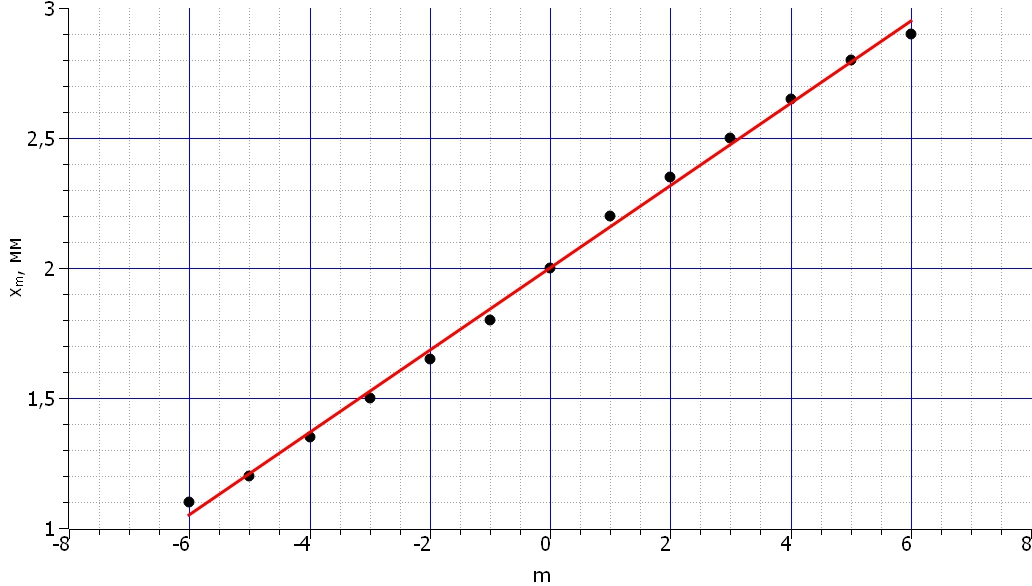
\includegraphics[scale=0.62]{Pictures/X(m)}
			\caption{Зависимость $x_m(m)$}
		\end{figure}
		
		По углу наклона прямой определим среднее расстояние между соседними минимумами: $\Delta X = (0,160 \pm 0,003)$ мм. 
		
		По формуле 
		\begin{equation*}
			D = \lambda \frac{f_2}{\Delta X}
		\end{equation*}
	
		определим ширину щели: $D = (0,310 \pm 0,001)$ мм, что почти совпадает с определенным раньше значением.
	\end{enumerate}


	\section*{В. Дифракция Фраунгофера на двух щелях}
	
	Для наблюдения дифракции Фраунгофера на двух щелях в установке следует заменить щель $S_2$ экраном Э с двумя щелями. 
	
	Если входная щель достаточно узка, то дифракционная картина в плоскости $\Pi$ подобна той, что получалась при дифракции на одной щели, однако теперь вся картина испещрена рядом дополнительных узких полос. Наличие этих полос объясняется суперпозицией световых волн, приходящих в плоскость наблюдения через разные щели экрана Э.
	\begin{figure}[h!]
		\centering
		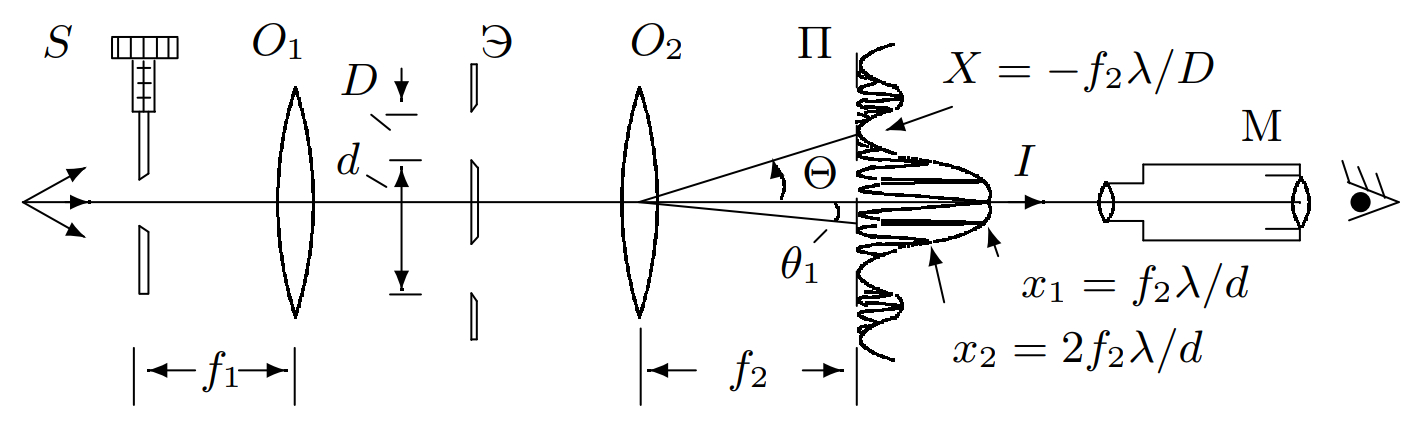
\includegraphics[scale=0.5]{Pictures/Double}
		\caption{Схема установки для наблюдения дифракции Фраунгофера на двух щелях}
	\end{figure}


	Линейное расстояние $\delta x$ между соседними интерференционными полосами в плоскости $\Pi$ равно:
	\begin{equation*}
		\delta x = f_2 \frac{\lambda}{d}.
	\end{equation*}

	Нетрудно оценить число $n$ интерференционных полос, укладывающихся в области центрального дифракционного максимума:
	\begin{equation*}
		n = \frac{2\lambda f_2}{D} \frac{1}{\delta x} = \frac{2d}{D}.
	\end{equation*}
	
	
	При дифракции света на двух щелях чёткая система интерференционных полос наблюдается только при достаточно узкой ширине входной щели $S$. При увеличении её ширины интерференционная картина периодически пропадает и появляется вновь, но полосы при этом оказываются сильно размытыми и видны плохо. Это явление объясняется наложением интерференционных картин от разных элементов широкой щели $S$. Первое размытие интерференционных полос возникает при условии:
	\begin{equation*}
		\frac{b}{f_1} = \frac{\lambda}{d}.
	\end{equation*}



	\begin{center}
		\textbf{I. Настройка и измерения}
	\end{center}
	
	\begin{enumerate}
		\item Не перемещая линз и микроскопа, заменим в установке входную щель $S_1$ щелью с микрометрическим винтом и, слегка передвигая её вдоль скамьи, найдем в микроскопе резкое изображение новой входной щели.
		
		Поставим между линзами экран Э с двойной щелью. В области главного дифракционного максимума появилась система равноотстоящих тёмных и светлых полос. Центрировкой системы и подбором ширины щели $S$ добьемся наибольшей чёткости дифракционной картины.
		
		\item Определим с помощью микрометрического винта поперечных салазок микроскопа координаты самых удалённых друг от друга тёмных полос внутри центрального максимума: $\Delta X = 0,7$ мм.
		Посчитаем число светлых промежутков между ними: $n = 9$. Измерим ширину центрального максимума: $\Delta L = 0,8$ мм.
		
		\item Исследуем влияние пространственной когерентности на видность интерференционной картины. Для этого, расширяя входную щель $S$, подберем такую ширину щели $b_0$, при которой наступает первое исчезновение интерференционных полос, и запишем эту величину: $b_0 = 0,31$ мм.
		
		Определим ширину, при которой картина наиболее контрастна: \\ $b_\text{max} = 0,27$ мм.
		
		\item Запишем фокусные расстояния обеих линз: $f_1 = 10,8$ см, $f_2 = 9$ см.
		
		
		
		\begin{center}
			\textbf{II. Обработка результатов}
		\end{center}
	
		\item Определим расстояние между минимумами: $\delta x = X / n = 0,078$ мм.
		
		Рассчитаем величину $d$:
		\begin{equation*}
			d = f_2 \frac{\lambda}{\delta x} = 0,9 \text{ мм.}
		\end{equation*}
		
		Рассчитаем число полос внутри главного максимума по формуле:
		\begin{equation*}
			n = \frac{2d}{D} = 8.
		\end{equation*}
	
		Почти совпадает с экспериментом.
		
		\item Сравним измеренную ширину $b_0$ щели $S$ с расчетом:
		\begin{equation*}
			b_0 = f_1 \frac{\lambda}{d} = 0,4 \text{ мм.}
		\end{equation*}
		
		Достаточно сильно расходится с измеренным значением.
	\end{enumerate}


	\section*{Г. Влияние дифракции на разрешающую способность оптического инструмента}
	
	Линзы $O_1$ и $O_2$ в отсутствие щели $S_2$ создают в плоскости $\Pi$ изображение щели $S_1$, и это изображение рассматривается в микроскоп $M$. Таким образом, нашу установку можно рассматривать как оптический инструмент, предназначенный для получения изображения предмета.
	
	Если перед объективом $O_2$ зрительной трубы расположить щель $S_2$, то изображение объекта будет искажено дифракцией на щели $S_2$. Чем меньше ширина $D_0$ этой щели, тем сильнее искажение.

	\begin{figure}[h!]
		\centering
		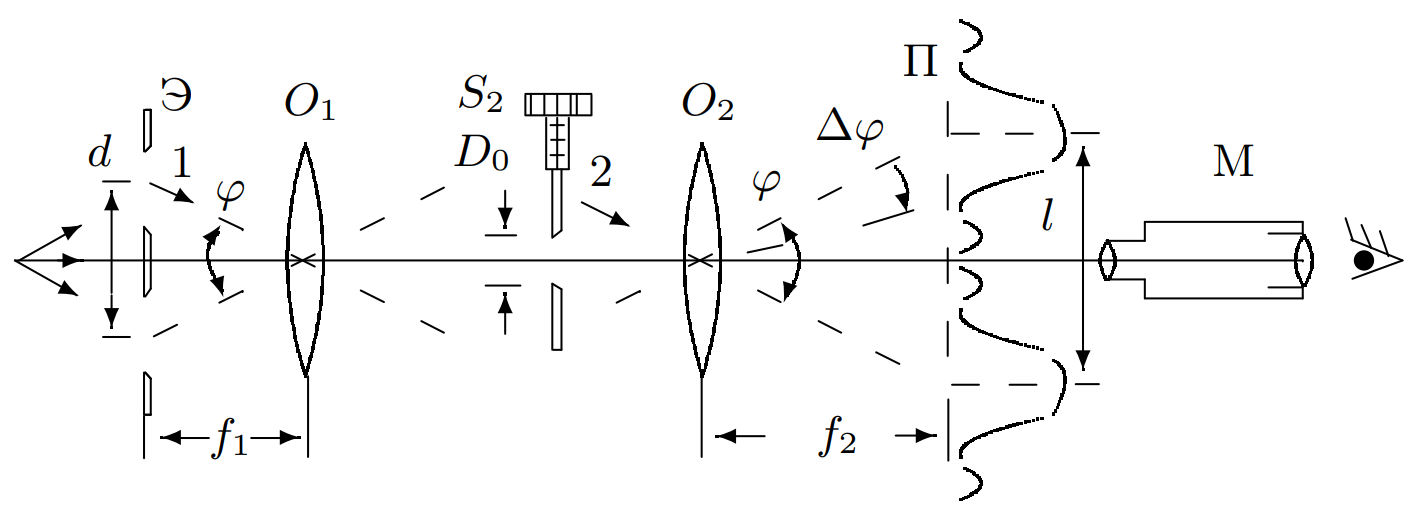
\includegraphics[scale=0.5]{Pictures/Rasr}
		\caption{Схема установки для исследования разрешающей способности оптического инструмента}
	\end{figure}

	Из критерия Рэлея получаем:
	\begin{equation*}
		\frac{\lambda}{D_0} = \frac{d}{f_1}.
	\end{equation*}

	
	\begin{center}
		\textbf{I. Настройка и измерения}
	\end{center}

	\begin{enumerate}
		\item Соберем схему согласно рисунку. Для этого в предыдущей схеме, не меняя положения линз и микроскопа, вместо щели $S$ поставим
двойную щель и, перемещая её вдоль оси, получим в поле зрения микроскопа чёткое, симметричное изображение двойного источника.
		
		\item Поставим между линзами щель $S_2$ и, уменьшая её ширину, наблюдаем за ухудшением качества изображения. Подберем ширину щели $S_2$ так, чтобы изображения обеих щелей почти сливались, но всё-таки ещё воспринимались раздельно. Запишем показания микрометрического винта щели $S_2$: $D_0 = 0,06$ мм.
		
		\item Поставим двойную щель перед микроскопом и измерим с помощью микрометрического винта поперечных салазок микроскопа расстояние $d$ между щелями: $d = 0,7$ мм. А также ширину каждой щели: $D = 0,06$ мм.
		
		
		\begin{center}
			\textbf{II. Обработка результатов}
		\end{center}
	
		\item Для проверки справедливости критерия Рэлея сравните измеренную ширину $D_0$ щели $S_2$ с расчётом: $D_0 = \lambda f_1 / d = 0,08$ мм, что недалеко от измеренного значения.
	\end{enumerate}
	
	
	\vspace{15mm}
	\section*{Вывод}
	В данной работе мы пронаблюдали и исследовали дифракцию Френеля и Фраунгофера, а также изучили влияние дифракции на разрешающую способность оптических инструментов. В ходе работы были определены некоторые величины, специфичные для эксперимента -- в них присутствуют погрешности. Они связаны с несовершенством техники измерения.

	
\end{document}